% This file was created with tikzplotlib v0.10.1.
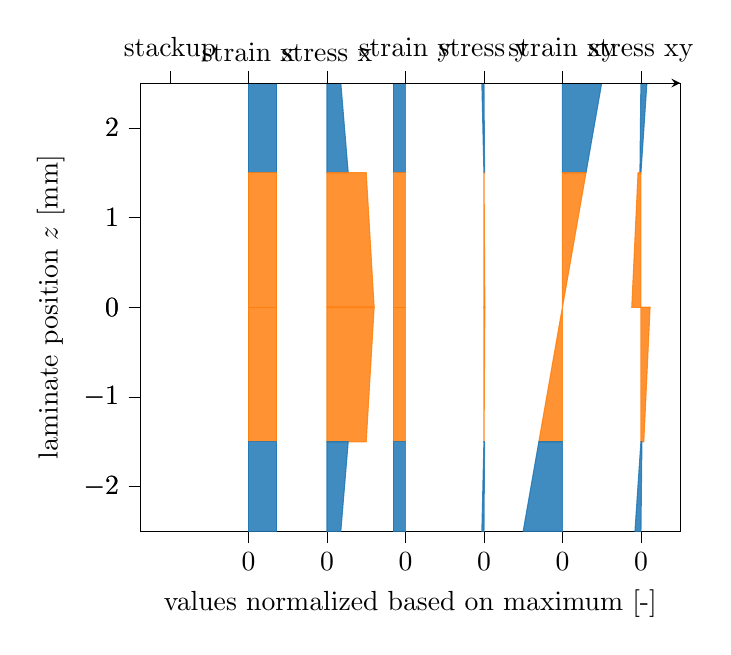
\begin{tikzpicture}

\definecolor{darkgray176}{RGB}{176,176,176}
\definecolor{darkorange25512714}{RGB}{255,127,14}
\definecolor{steelblue31119180}{RGB}{31,119,180}

\begin{axis}[
tick align=outside,
tick pos=left,
x grid style={darkgray176},
xlabel={values normalized based on maximum [-]},
xmin=-0.75, xmax=13,
xtick style={color=black},
xtick={2,4,6,8,10,12},
xticklabels={0,0,0,0,0,0},
y grid style={darkgray176},
ylabel={laminate position \(\displaystyle z\) [mm]},
ymin=-2.5, ymax=2.5,
ytick style={color=black}
]
\path [draw=steelblue31119180, fill=steelblue31119180, opacity=0.85]
(axis cs:2,2.5)
--(axis cs:2.72481350038477,2.5)
--(axis cs:2.72481350038477,1.5)
--(axis cs:2,1.5)
--cycle;
\path [draw=steelblue31119180, fill=steelblue31119180, opacity=0.85]
(axis cs:4,2.5)
--(axis cs:4.35255663184007,2.5)
--(axis cs:4.54136852083958,1.5)
--(axis cs:4,1.5)
--cycle;
\path [draw=steelblue31119180, fill=steelblue31119180, opacity=0.85]
(axis cs:5.68876168547323,2.5)
--(axis cs:6,2.5)
--(axis cs:6,1.5)
--(axis cs:5.68876168547323,1.5)
--cycle;
\path [draw=steelblue31119180, fill=steelblue31119180, opacity=0.85]
(axis cs:7.94759925769598,2.5)
--(axis cs:8,2.5)
--(axis cs:8.01588767461782,1.5)
--(axis cs:8,1.5)
--cycle;
\path [draw=steelblue31119180, fill=steelblue31119180, opacity=0.85]
(axis cs:10,2.5)
--(axis cs:11,2.5)
--(axis cs:10.6,1.5)
--(axis cs:10,1.5)
--cycle;
\path [draw=steelblue31119180, fill=steelblue31119180, opacity=0.85]
(axis cs:12,2.5)
--(axis cs:12.1517399718851,2.5)
--(axis cs:12,1.5)
--(axis cs:11.9754445487355,1.5)
--cycle;
\path [draw=darkorange25512714, fill=darkorange25512714, opacity=0.85]
(axis cs:2,1.5)
--(axis cs:2.72481350038477,1.5)
--(axis cs:2.72481350038477,0)
--(axis cs:2,0)
--cycle;
\path [draw=darkorange25512714, fill=darkorange25512714, opacity=0.85]
(axis cs:4,1.5)
--(axis cs:5,1.5)
--(axis cs:5.20172030218258,0)
--(axis cs:4,0)
--cycle;
\path [draw=darkorange25512714, fill=darkorange25512714, opacity=0.85]
(axis cs:5.68876168547323,1.5)
--(axis cs:6,1.5)
--(axis cs:6,0)
--(axis cs:5.68876168547323,0)
--cycle;
\path [draw=darkorange25512714, fill=darkorange25512714, opacity=0.85]
(axis cs:8,1.5)
--(axis cs:8.00170347552903,1.5)
--(axis cs:8.0226385695951,0)
--(axis cs:8,0)
--cycle;
\path [draw=darkorange25512714, fill=darkorange25512714, opacity=0.85]
(axis cs:10,1.5)
--(axis cs:10.6,1.5)
--(axis cs:10,0)
--(axis cs:10,0)
--cycle;
\path [draw=darkorange25512714, fill=darkorange25512714, opacity=0.85]
(axis cs:11.9272437545994,1.5)
--(axis cs:12,1.5)
--(axis cs:12,0)
--(axis cs:11.7671770084466,0)
--cycle;
\path [draw=darkorange25512714, fill=darkorange25512714, opacity=0.85]
(axis cs:2.72481350038477,0)
--(axis cs:2,0)
--(axis cs:2,-1.5)
--(axis cs:2.72481350038477,-1.5)
--cycle;
\path [draw=darkorange25512714, fill=darkorange25512714, opacity=0.85]
(axis cs:4,0)
--(axis cs:5.20172030218258,0)
--(axis cs:5,-1.5)
--(axis cs:4,-1.5)
--cycle;
\path [draw=darkorange25512714, fill=darkorange25512714, opacity=0.85]
(axis cs:6,0)
--(axis cs:5.68876168547323,0)
--(axis cs:5.68876168547323,-1.5)
--(axis cs:6,-1.5)
--cycle;
\path [draw=darkorange25512714, fill=darkorange25512714, opacity=0.85]
(axis cs:8,0)
--(axis cs:8.0226385695951,0)
--(axis cs:8.00170347552903,-1.5)
--(axis cs:8,-1.5)
--cycle;
\path [draw=darkorange25512714, fill=darkorange25512714, opacity=0.85]
(axis cs:10,0)
--(axis cs:10,0)
--(axis cs:9.4,-1.5)
--(axis cs:10,-1.5)
--cycle;
\path [draw=darkorange25512714, fill=darkorange25512714, opacity=0.85]
(axis cs:12,0)
--(axis cs:12.2328229915534,0)
--(axis cs:12.0727562454006,-1.5)
--(axis cs:12,-1.5)
--cycle;
\path [draw=steelblue31119180, fill=steelblue31119180, opacity=0.85]
(axis cs:2.72481350038477,-1.5)
--(axis cs:2,-1.5)
--(axis cs:2,-2.5)
--(axis cs:2.72481350038477,-2.5)
--cycle;
\path [draw=steelblue31119180, fill=steelblue31119180, opacity=0.85]
(axis cs:4,-1.5)
--(axis cs:4.54136852083958,-1.5)
--(axis cs:4.35255663184007,-2.5)
--(axis cs:4,-2.5)
--cycle;
\path [draw=steelblue31119180, fill=steelblue31119180, opacity=0.85]
(axis cs:6,-1.5)
--(axis cs:5.68876168547323,-1.5)
--(axis cs:5.68876168547323,-2.5)
--(axis cs:6,-2.5)
--cycle;
\path [draw=steelblue31119180, fill=steelblue31119180, opacity=0.85]
(axis cs:8,-1.5)
--(axis cs:8.01588767461782,-1.5)
--(axis cs:8,-2.5)
--(axis cs:7.94759925769598,-2.5)
--cycle;
\path [draw=steelblue31119180, fill=steelblue31119180, opacity=0.85]
(axis cs:10,-1.5)
--(axis cs:9.4,-1.5)
--(axis cs:9,-2.5)
--(axis cs:10,-2.5)
--cycle;
\path [draw=steelblue31119180, fill=steelblue31119180, opacity=0.85]
(axis cs:12,-1.5)
--(axis cs:12.0245554512645,-1.5)
--(axis cs:12,-2.5)
--(axis cs:11.8482600281149,-2.5)
--cycle;
\end{axis}

\begin{axis}[
axis x line=top,
legend cell align={left},
legend style={fill opacity=0.8, draw opacity=1, text opacity=1, at={(1.05,0.5)}, anchor=west, draw=none},
tick align=outside,
x grid style={darkgray176},
xmin=-0.75, xmax=13,
xtick pos=right,
xtick style={color=black},
xtick={0,2,4,6,8,10,12},
xticklabels={stackup,strain x,stress x,strain y,stress y,strain xy,stress xy},
y grid style={darkgray176},
ymin=-2.5, ymax=2.5,
ytick pos=left,
ytick style={color=black}
]
\end{axis}

\end{tikzpicture}
